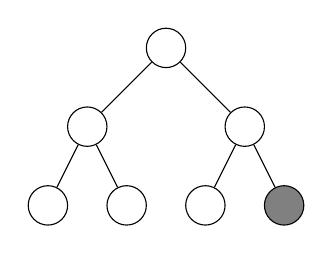
\begin{tikzpicture}
\tikzstyle{tnode}=[circle,draw,minimum width=0.5cm];
\tikzstyle{dnode}=[tnode,fill=gray];

\node [tnode] (v1) at (0,2) {};
\node [tnode] (v2) at (-1,1) {};
\node [tnode] (v5) at (1,1) {};
\node [tnode] (v3) at (-1.5,0) {};
\node [tnode] (v4) at (-0.5,0) {};
\node [tnode] (v6) at (0.5,0) {};
\node [dnode] (v7) at (1.5,0) {};
\draw  (v1) edge (v2);
\draw  (v2) edge (v3);
\draw  (v2) edge (v4);
\draw  (v1) edge (v5);
\draw  (v5) edge (v6);
\draw  (v5) edge (v7);
\end{tikzpicture}